\section{Konzept (H.L.)}
\label{sec-Konzept}

Durch unsere Teamzusammensetzung und unser Vorwissen haben wir uns für diesen Projektaufbau entschieden.
Dies war vorteilhaft, da wir parallel anfangen konnten zu arbeiten, ohne auf die anderen warten zu müssen.
Die beruflichen Kenntnisse und Aufgaben haben uns in vielen Bereichen geschult und vorbereitet. 
Das Vorwissen was wir zusammen einbrachten ist weit gestreut in den Bereichen C\#, Webentwicklung, APIs oder Docker.
Diese Projektarbeit hat uns die Chance geboten viel von diesen Fähigkeiten abzurufen und anzuwenden.
Unsere Methoden und der Umgang mit dem Material der Daten bot großes Potenzial erneut an diesen Fähigkeiten zu feilen.
Zusätzlich lernten wir viele neue Wege und Methoden, um so eine Aufgabe zu bewältigen.
So entstand die Idee für diese Projektskizze.

\begin{figure}[H]
    \centering
    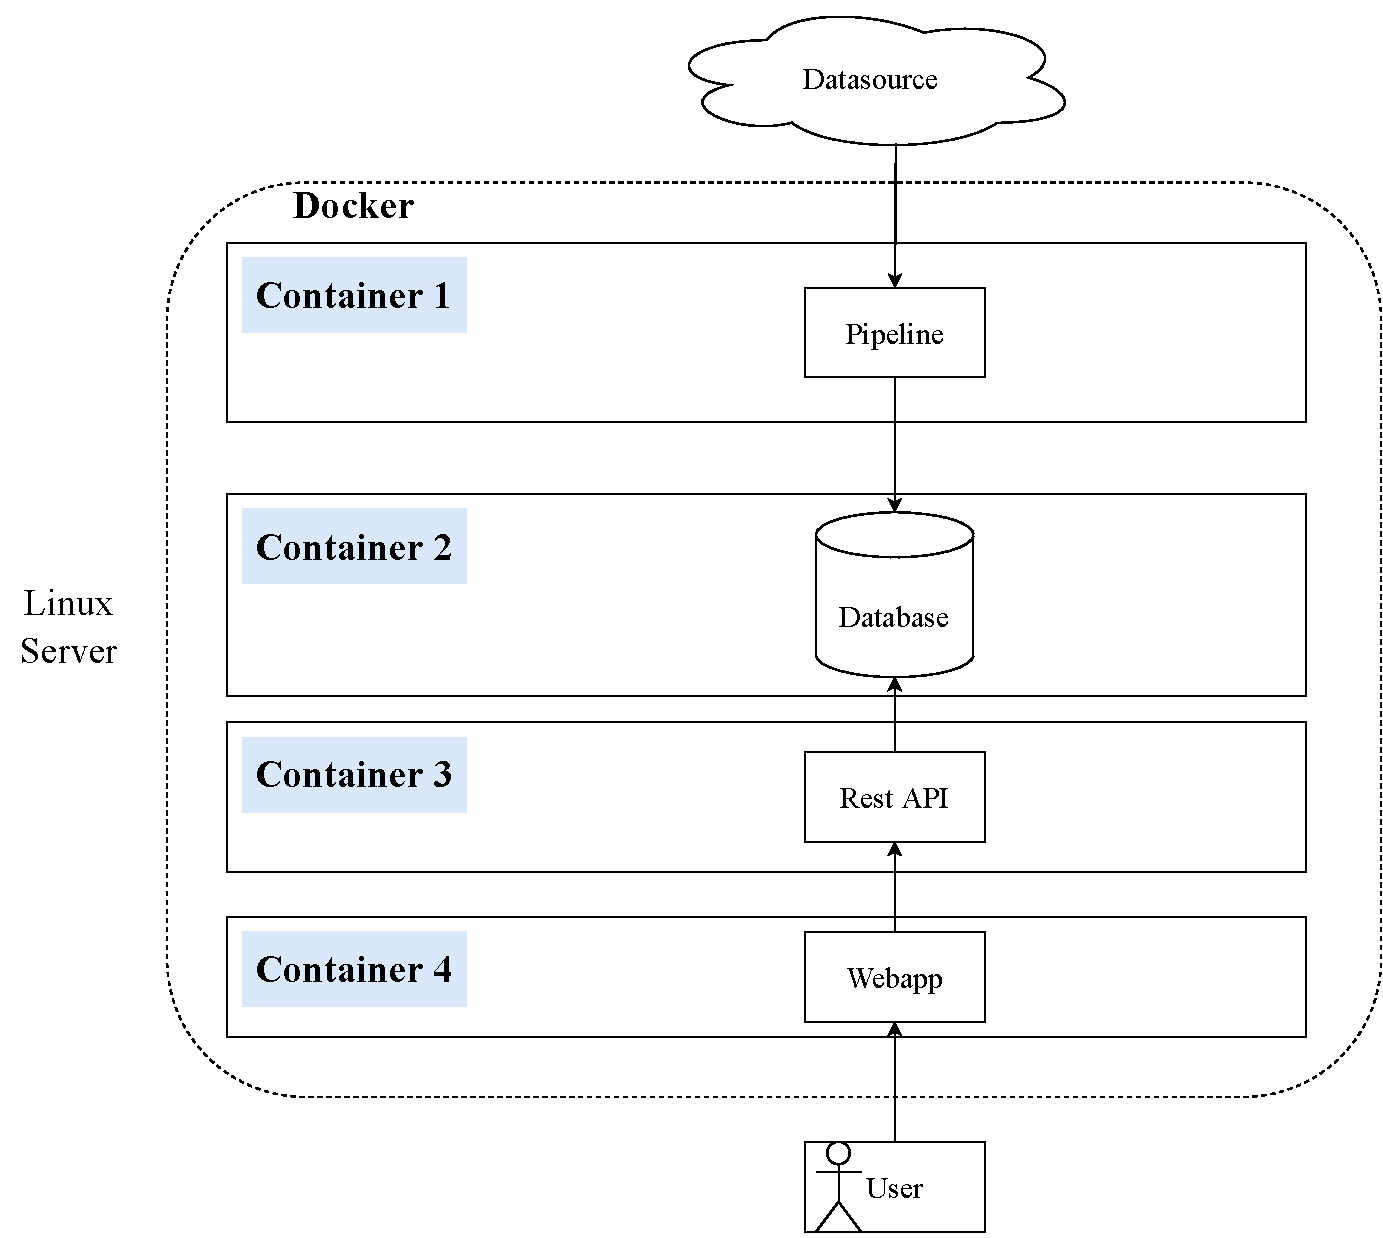
\includegraphics[width=8cm]{figures/method.pdf}
    \caption{Skizze unseres Konzeptes}
    \label{fig:Skizze unserer Idee}
\end{figure}
